\chapter{Architectural Design}
This section aims to present and analyze the architecture of the S2B in a top-down manner. 
We discuss about the architectural design choices and the reasons behind them. 

\section{Overview: High-level components and their interactions}
The figure shown below represents a high-level description of the components which make up the system.
\begin{figure}[H]
    \centering
    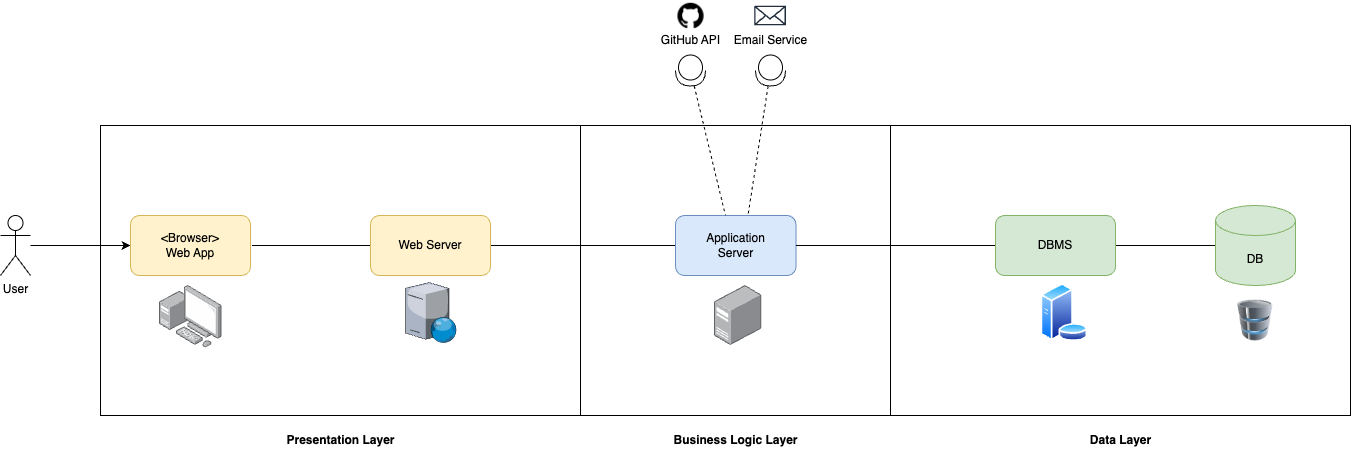
\includegraphics[width=\textwidth]{images/component_view/high_level.png}
    \caption{Overview CKB architecture}
    \label{fig:CKB Architecture}
\end{figure}
A web interface will be used to access the platform. 
The overall architecture of the system is based on a three-tier architecture, 
with the application servers interacting with a database management system and
using APIs to retrieve and store data. \\
The three logical layers corrspond to three different physical layers and each layer can communicate only with the adjacent ones.
The interactions between clients and server are stateless according to the REST architectural style. \\
The web server is responsible for the communication with the clients and for the management of the requests. \\
The application server holds the business logic of the application and it can communicate with the database server to retrieve and store data, also with the GitHub platform and the Email Service. 

\section{Component view}
\begin{figure}[H]
    \centering
    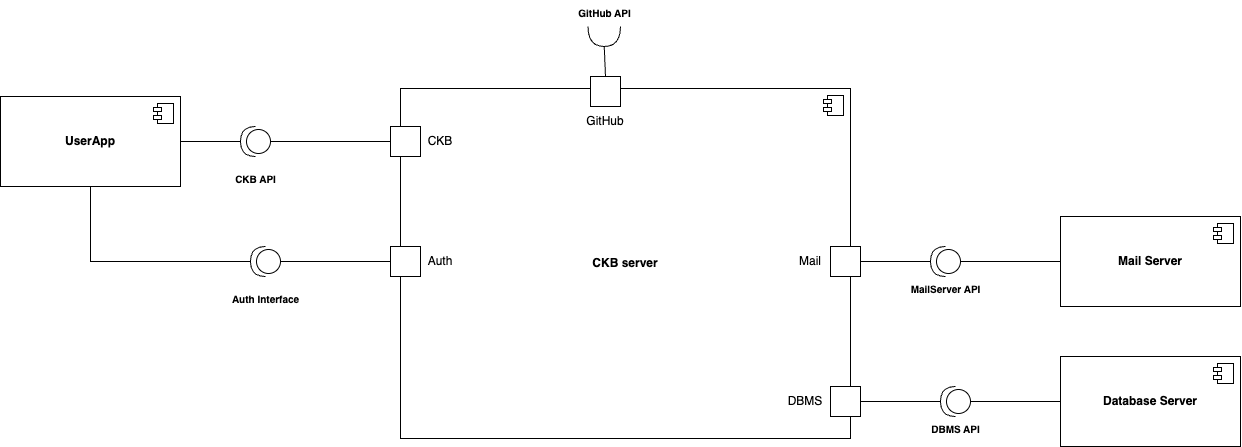
\includegraphics[width=\textwidth]{images/component_view/Component_view.png}
    \caption{High level component view}
\end{figure}

\begin{figure}[H]
    \centering
    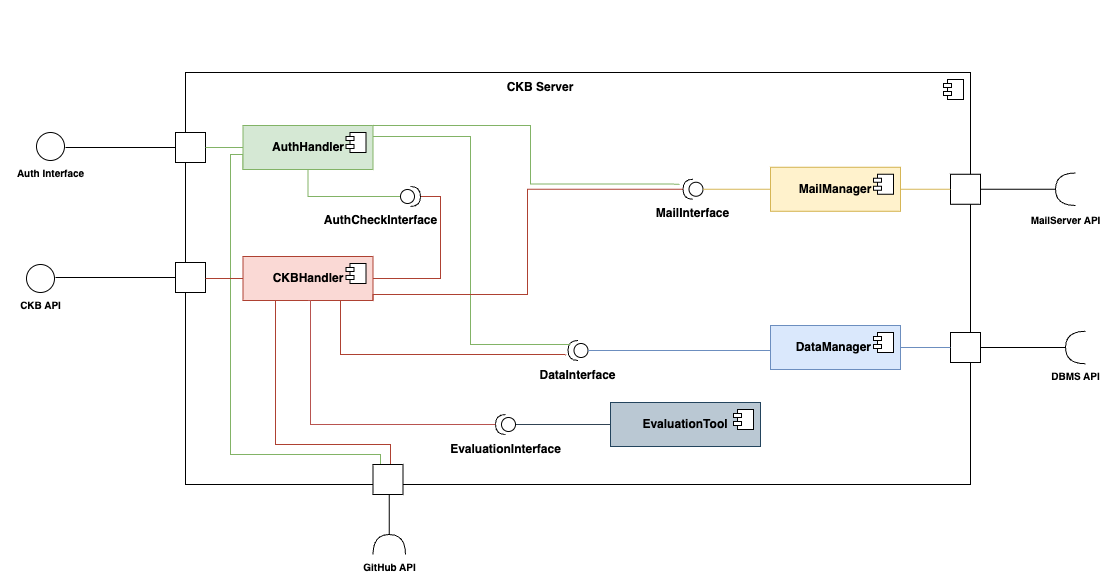
\includegraphics[width=\textwidth]{images/component_view/CKB_component.png}
    \caption{CKB server component view}
\end{figure}

\begin{figure}[H]
    \centering
    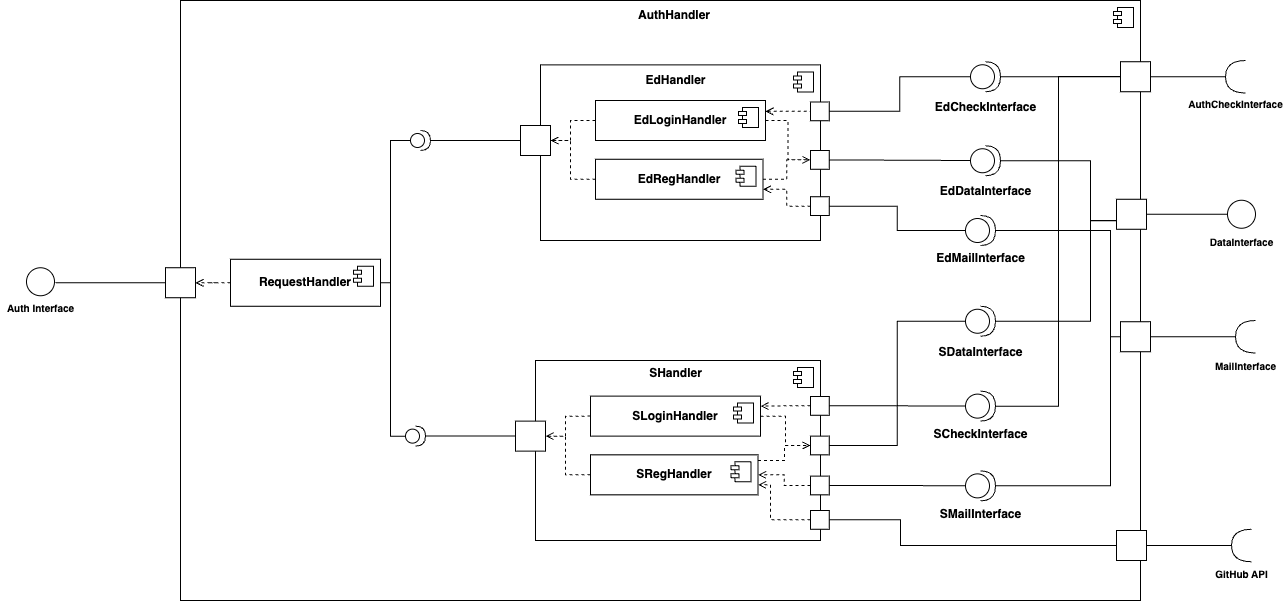
\includegraphics[width=\textwidth]{images/component_view/Auth.png}
    \caption{Auth component view}
\end{figure}

\section{Deployment view}
\section{Runtime view}
\section{Component interfaces}
\section{Selected architetural styles and patterns}
\section{Other design decisions}